\documentclass[10pt]{beamer}

\usetheme[progressbar=frametitle]{Madrid}
\usepackage{appendixnumberbeamer}

\usepackage{booktabs}
\usepackage[scale=2]{ccicons}
\usepackage{diagbox}
\usepackage{pifont}
\newcommand{\cmark}{\ding{51}}
\newcommand{\xmark}{\ding{55}}

\usepackage{pgfplots}
\usepgfplotslibrary{dateplot}
\usepackage{amssymb,amsmath}

\usepackage{xspace}
\usepackage{multirow}
\usepackage[ruled, linesnumbered]{algorithm2e}
\usepackage{multimedia}
\usepackage{media9}
\newcommand{\includemovie}[3]{%
\includemedia[%
width=#1,height=#2,%
activate=pagevisible,%
deactivate=pageclose,%
addresource=#3,%
flashvars={%
src=#3 % same path as in addresource!
&autoPlay=true % default: false; if =true, automatically starts playback after activation (see option ‘activation)’
&loop=true % if loop=true, media is played in a loop
&controlBarAutoHideTimeout=0 %  time span before auto-hide
}%
]{}{StrobeMediaPlayback.swf}%
}% end of the new command

% For caption without labels
\usepackage{caption}
\captionsetup{font=tiny}
\setbeamertemplate{caption}{\raggedright\insertcaption\par}

\newcommand{\lv}{\lVert}
\newcommand{\rv}{\rVert}

\AtBeginSection{%
\begin{frame}
    \tableofcontents[currentsection, subsectionstyle=show/show/hide]
\end{frame}
}


\title{Multi-fidelity enhanced neural network modeling }

\date{Nov 15, 2019}
\author[Chuan Lu]{Chuan Lu \\[5pt]
Advisor: Prof. Xueyu Zhu}
\institute[AMCS]{Applied Mathematical and Computational Sciences, University of Iowa}

\titlegraphic{\hfill
\includegraphics[height=1.5cm]{DomeWordPrimaryBLACK.eps}}

\begin{document}
\maketitle


\begin{frame}
\tableofcontents
\end{frame}

\section{Introduction}

\begin{frame}{High-fidelity simulations}
Parameterized PDE:
\nocite{maday2006reduced}
\nocite{hesthaven2018non}
\nocite{zhu2014computational}
\nocite{lu2019bifidelity}

$$
\left\{
\begin{aligned}
&\mathcal{L}(x, z)u(x, z) = f(x, z), \quad \text{in}\ D(z), \\ 
&u(x, z) = g(x, z), \quad \text{on}\ \partial D(z).
\end{aligned}
\right.
$$
\begin{itemize}
	\item Indispensible in science and engineering
	\item High accuracy requires high computational cost
	\item Many-query problems: solve the PDE for $z \in Z_{query} \subset I_{z} $.
\end{itemize}


\begin{figure}
\centering
  \begin{minipage}[t]{0.32\textwidth}
    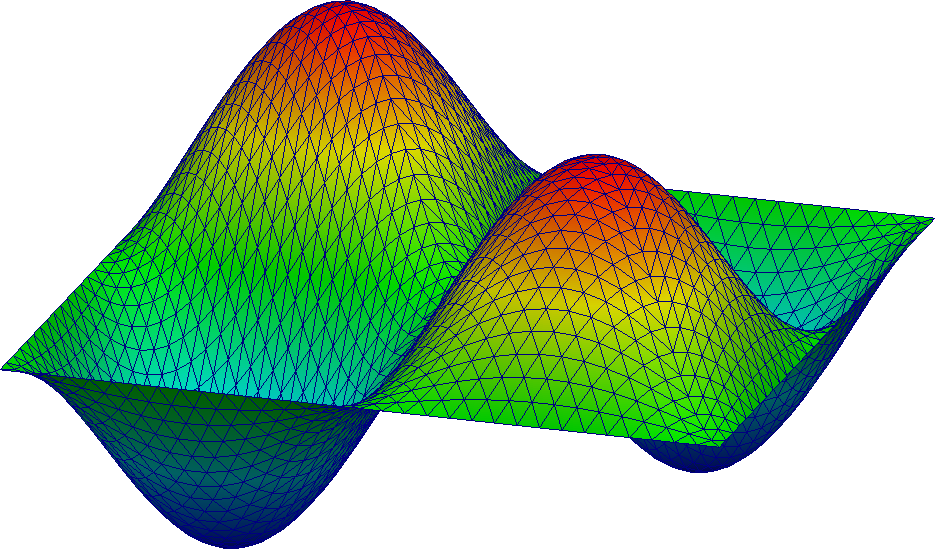
\includegraphics[width=\textwidth]{Figures/introduction/Lapl2D_4.png}
    \footnotemark[1]
    \caption{2D Laplace equation}
  \end{minipage}
  \begin{minipage}[t]{0.32\textwidth}
    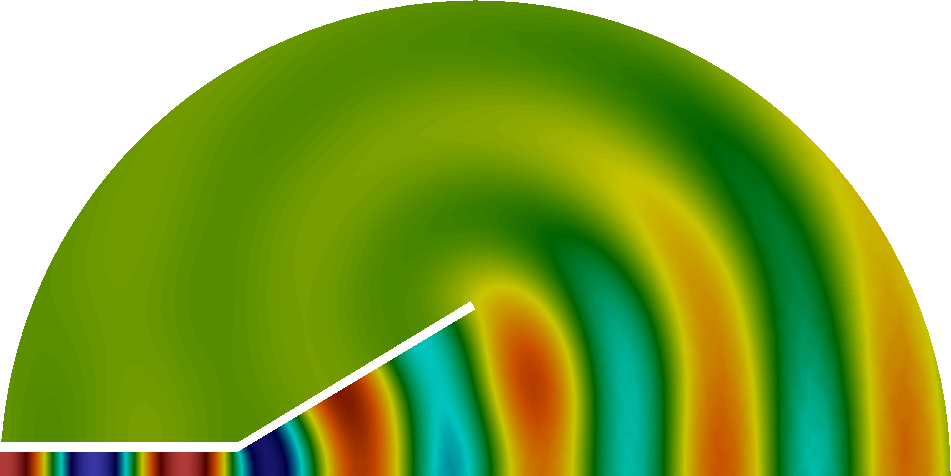
\includegraphics[width=\textwidth]{Figures/introduction/AcousticHorn.png}
    \footnotemark[1]
    \caption{2D Helmholtz equation}
  \end{minipage}
  \begin{minipage}[t]{0.32\textwidth}
    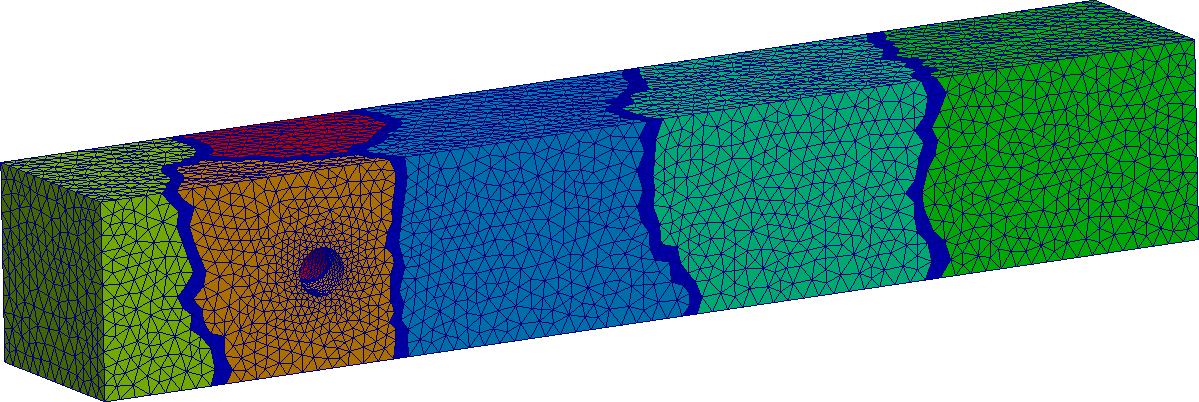
\includegraphics[width=\textwidth]{Figures/introduction/Dfg3D_DD_2.png}
    \footnotemark[1]
    \caption{3D Navier-Stokes equation}
  \end{minipage}
\end{figure}
\footnotetext[1]{\tiny A. Quarteroni, A. Manzoni and F. Negri.
Reduced Basis Methods for Partial Differential Equations. An Introduction.
Unitext, vol. 92. Springer, 2016. https://redbkit.github.io/redbKIT/}
\end{frame}

\begin{frame}{Reduced Basis Methods (RBM)}
\begin{itemize}
\item Target: Compute the desired output {\color{red} accurately} and at {\color{red} minimal} cost \cite{maday2006reduced}.
$$
z \xrightarrow{\mathcal{\tilde{L}}} u(x; z)
$$
\item Central idea: Identify a problem-dependent basis to represent solutions of PDEs.
\item Dominating method: Proper Orthogonal Decomposition (POD) \cite{hesthaven2016certified}.
\end{itemize}
\end{frame}

\begin{frame}{POD}
POD seeks for a set of basis $\{\varphi_i\}_{i=1}^n $ that minimizes the quantity \cite{hesthaven2016certified}
\begin{equation}
\sqrt{\frac{1}{M} \sum_{z \in Z} \inf_{v\in V_{rb}} \lv u(z) - v\rv^2},
\end{equation}
where $V_{rb} = \text{span}\{\varphi_i\} \subset \text{span}\{u(z) \mid z\in Z\}$, $Z$ is the discrete parameter set where the {\color{red} snapshots} $u(z)$ are evaluated.
\begin{itemize}
	\item Minimize the distance to all collected snapshots
	\item Equivalent to singular value decomposition (SVD) in Euclidean space
\end{itemize}
\end{frame}

\begin{frame}{POD}
\begin{enumerate}
	\item Select a collection of parameters $\Gamma \subset I_z $, and generate the snapshots $u(z_i)$ for each $z_i \in \Gamma $.
	\item Perform a SVD on the snapshot matrix $S = [u(z_i)]$:
	\begin{equation}
		S = U\Sigma W^\top.
	\end{equation}
	\item For a chosen dimension $r$, pick the first $r$ left singular vectors to form the POD basis $V$.
	\item The reduced representation are computed by 
	\begin{equation}
		u_r(z) = Vc_r(z),
	\end{equation}
	here $c_r(z) $ is the POD coefficients computed by
	\begin{equation}
		c_r(z) = V^\top u(z).
	\end{equation}
\end{enumerate}
\end{frame}

\begin{frame}{Nonintrusive RBM}
How to compute the POD approximation of a solution $u(z)$ with a {\color{red} new} parameter value $z$?\\[10pt]

Key: Compute the POD coefficient $c(z)$ for $u(z)$ {\color{red} without} solving the original PDE. \\[10pt]

Traditional solution: POD-Galerkin. Project the equation $\mathcal{L}(x, z)u(x, z) = f(x, z)$ onto the POD basis; Solve $Ac = b$ \cite{maday2006reduced,rozza2007reduced,buffa2012priori}.
\begin{itemize}
\item[\xmark] Need to rewrite the solver
\end{itemize}\\[10pt]

Nonintrusive: Build a surrogate to the coefficients and approximate $c(z)$ by interpolation over parameter space \cite{xiao2015non,xiao2016non,xiao2017parameterized,garotta2018reduced}.
\begin{itemize}
\item[\cmark] No need for rewriting solver
\item[\xmark] Prone to fail for complex problems
\end{itemize}
\end{frame}


\begin{frame}{POD-NN}
POD + neural networks \cite{hesthaven2018non}: \\[10pt]
\begin{itemize}
\item[\cmark] Use multilayer perceptrons (MLP) to approximate the POD coefficients, with the parameter as the input
\item[\cmark] Provide a data-driven approach instead of using nonadapted interpolation basis set
\item[\cmark] Has a superior performance than POD-Galerkin based methods for nonlinear parameterized problems
\item[\xmark] The input features are just parameters of the physical model, which are not strongly informative
\end{itemize}
\\[10pt]
If {\color{red} better} features are provided to the neural networks, we can expect better approximation accuracy with {\color{red} limited} data.
\end{frame}

\begin{frame}{Low-fidelity models}
Low-fidelity models \cite{alexandrov2000optimization,sun2011multi,cutler2014reinforcement}:
\begin{itemize}
	\item[\cmark] Common in practical problems (e.g. coarser mesh)
	\item[\cmark] Cheap to compute
	\item[\cmark] Inaccurate, but can still mimic important behaviors of the problem
\end{itemize}
\end{frame}

\begin{frame}{BiFi-NN}
When a cheap low-fidelity model and expensive high-fidelity model are available \cite{lu2019bifidelity}:
\begin{itemize}
	\item[\cmark] Still use MLPs to approximate high-fidelity POD coefficients
	\item[\cmark] {\color{red} Extend input} with features extracted from low-fidelity model
	\item[\cmark] Better approximation accuracy with {\color{red} limited data}
	\item[\cmark] Remain nonintrusive 
	\item[\xmark] Additional computational cost in low-fidelity simulation
\end{itemize} 
\end{frame}


%%%%%%%%%%%%%%%%%%%%%%%%%%%%%%%%%%%%%%%%%%%%%%%%%%%%%%%%%%%%%%%%%%%%%%%%%%%%
%%%%%%%%%%%%%%%%%%%%%%%%%%%%%%%%%%%%%%%%%%%%%%%%%%%%%%%%%%%%%%%%%%%%%%%%%%%%
%%%%%%%%%%%%%%%%%%%%%%%%%%%%%%%%%%%%%%%%%%%%%%%%%%%%%%%%%%%%%%%%%%%%%%%%%%%%
%%%%%%%%%%%%%%%%%%%%%%%%%%%%%%%%%%%%%%%%%%%%%%%%%%%%%%%%%%%%%%%%%%%%%%%%%%%%
%%%%%%%%%%%%%%%%%%%%%%%%%%%%%%%%%%%%%%%%%%%%%%%%%%%%%%%%%%%%%%%%%%%%%%%%%%%%

\section{Methods}

\begin{frame}{Problem setup re-visit}
Parameterized PDE:
$$
\left\{
\begin{aligned}
&\mathcal{L}(x, z)u(x, z) = f(x, z), \quad \text{in}\ D(z), \\ 
&u(x, z) = g(x, z), \quad \text{on}\ \partial D(z).
\end{aligned}
\right.
$$
\begin{itemize}
	\item High-fidelity solution $u_h(x, z): D\times I_z \to \mathbb{V}_h $
	\item Low-fidelity solution  $u_l(x, z): D\times I_z \to \mathbb{V}_l $
\end{itemize}
\\[10pt]

Target: To compute the high-fidelity POD coefficients $c_h(z) $ for the high-fidelity solution $u_h(x, z) $.
\end{frame}


\subsection{POD-NN}

\begin{frame}{POD-NN}

Use neural networks to learn the mapping $\Phi: z \to c_h(z) $.

\begin{figure}
\centering
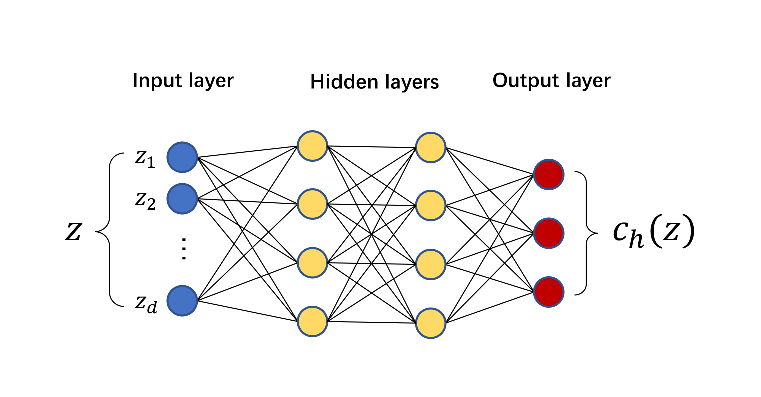
\includegraphics[scale=0.8]{Figures/method/PODNN.pdf}
\caption{Structure of PODNN.}
\label{PODNN-structure}
\end{figure}
\end{frame}


\subsection{BiFi-NN using low-fidelity POD coefficients}

\begin{frame}{BiFi-NN (first approach)}
Suppose there is a low-fidelity model $u_l(x; z) $ available in addition to the high-fidelity model $u_h(x; z) $. \\[10pt]

Our first approach is to use the whole low-fidelity POD coefficient vector $c_l(z) = [c_{l,1}(z), \cdots, c_{l, r}(z)]$ as the augmented data-dependent features: \\[10pt]
\begin{equation}
\Phi: (z; c_l(z)) \to  c_{h,i}(z).
\end{equation}
\begin{figure}
\centering
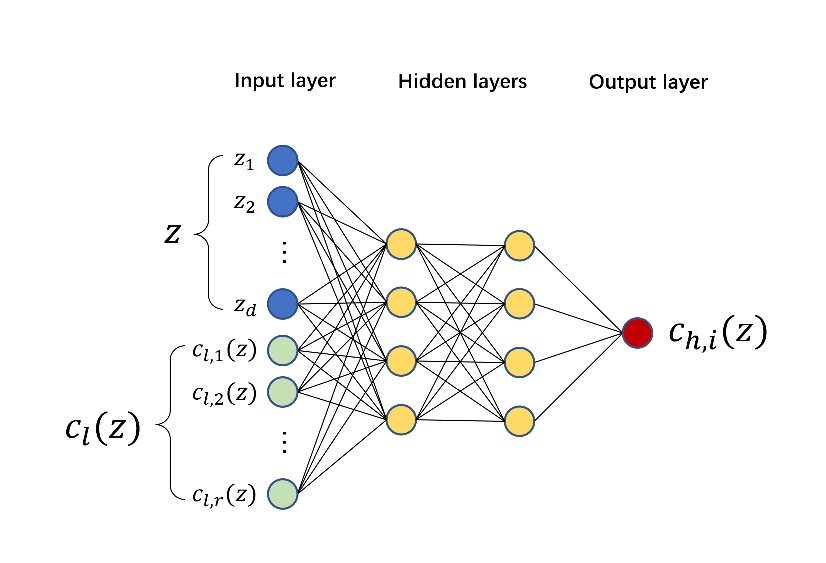
\includegraphics[scale=0.5]{Figures/method/BFNN.pdf}
\caption{Structure of BiFiNN (first approach).}
\label{BiFiNN-structure}
\end{figure}
\end{frame}

\begin{frame}{BiFi-NN (second approach)}
\begin{figure}
\centering
\includegraphics[scale=0.8]{Figures/method/BFNN-1.pdf}
\caption{Structure of BiFiNN (second approach).}
\label{BiFiNN-structure}
\end{figure}
\end{frame}

\begin{frame}{Lid-driven Cavity}

Low-fidelity POD basis and high-fidelity POD basis have different directions:

\begin{figure}
\centering
\vbox{
	\includegraphics[scale=0.15]{Figures/example13/u/pod/highfi_pod_1.pdf}
	\includegraphics[scale=0.15]{Figures/example13/u/pod/highfi_pod_2.pdf}
	\includegraphics[scale=0.15]{Figures/example13/u/pod/highfi_pod_3.pdf}
	\includegraphics[scale=0.15]{Figures/example13/u/pod/highfi_pod_4.pdf}
	\includegraphics[scale=0.15]{Figures/example13/u/pod/highfi_pod_5.pdf}
	\\
	\includegraphics[scale=0.15]{Figures/example13/u/pod/lowfi_pod_1.pdf}
	\includegraphics[scale=0.15]{Figures/example13/u/pod/lowfi_pod_2.pdf}
	\includegraphics[scale=0.15]{Figures/example13/u/pod/lowfi_pod_3.pdf}
	\includegraphics[scale=0.15]{Figures/example13/u/pod/lowfi_pod_4.pdf}
	\includegraphics[scale=0.15]{Figures/example13/u/pod/lowfi_pod_5.pdf}
}
\caption{Top: First 5 POD basis for high-fidelity solution; Bottom: First 5 POD basis for low-fidelity solution.}
\end{figure}

\end{frame}

\subsection{BiFi-NN using Bi-fidelity POD coefficients}

\begin{frame}{Bi-fidelity Surrogate}
Constructed as a linear combination of high-fidelity solutions on a selected set of parameter values. The selection of these ``important'' points is inferred by the low-fidelity snapshots \cite{zhu2014computational}.

\begin{figure}
\centering
\includegraphics[scale=0.35]{Figures/method/bifinn_diagram-1.pdf}
\caption{Flow chart of constructing a bi-fidelity surrogate.}
\label{BiFiNN-structure}
\end{figure}

\end{frame}

\begin{frame}{Cholesky Selection}
\begin{itemize}
	\item Main idea: Select ``important'' parameter values from the low-fidelity solutions
	\item Search iteratively for a new $z_k $ to maximize the distance between $u_l(z_k)$ and $\text{span}\{u_l(z_i)\mid i < k \}$.
	\item Coefficient $c_{bf}(z) $ obtained by projection to the {\color{red} low-fidelity basis}:
	\begin{equation}
		Gc_{bf}(z) = V_l(\gamma)^\top u_l(z)
	\end{equation}
	\item Accomplished by column pivoting in Cholesky factorization of the Gramiam matrix $G = [(u(z_i), u(z_j))]_{ij} $ of low-fidelity solutions.
\end{itemize}
\begin{figure}
\centering
\includegraphics[scale=0.35]{Figures/method/bifinn_diagram-1.pdf}
\caption{Flow chart of constructing a bi-fidelity surrogate.}
\label{BiFiNN-structure}
\end{figure}


\end{frame}

\begin{frame}{BiFi-NN (third approach)}
Use the $i^{th} $ component of the POD coefficient of the {\color{red} bi-fidelity surrogate} as the augmented feature:

\begin{figure}
\centering
\includegraphics[scale=0.8]{Figures/method/BFNN-3.pdf}
\caption{Structure of BiFiNN (third approach).}
\label{BiFiNN-structure}
\end{figure}
\end{frame}

% \begin{frame}{BiFi-NN (third approach)}
% \begin{figure}
% \centering
% \includegraphics[scale=0.45]{Figures/method/bifinn_diagram-2.pdf}
% \caption{Flow chart for BiFi-NN.}
% \label{BiFiNN-flow-chart}
% \end{figure}
% \end{frame}

\begin{frame}{BiFi-NN, Offline}
\centering
\begin{algorithm}[H]
\caption{Offline stage for BiFi-NN}
{\small

Sample a collection of parameters $\Gamma\subset I_z $.

Run the low-fidelity model $u_l(z_j) $ and high-fidelity model $u_h(z_j)$ for each $z_j\in \Gamma $.

Compute the POD basis $V_h $ and POD coefficients $c_h(z_j) $ by projection:
$$
c_h(z_j) = V_h^\top u_h(z_j).
$$

Construct a bi-fidelity surrogate $u_{bf}(z_j) $ and the Gramiam matrix $G$, low-fidelity basis $\tilde{V_l}$ and high-fidelity basis $\tilde{V_h} $.

Compute the POD coefficients of the bi-fidelity surrogate by projection:
$$
c_b(z_j) = V_h^\top u_{bf}(z_j).
$$

For each $i = 1, \hdots, r$, train a network $y = \Phi_i(x; \theta) $ with input $x = (z_j, c_{b,i}(z_j))$ and output $y = c_{h,i}(z_j) $.

}
\end{algorithm}
\end{frame}

\begin{frame}{BiFi-NN, Online}
\begin{algorithm}[H]
\caption{Online stage for BiFi-NN}
{\small

Run the low-fidelity model $u_l(z^*) $ for the given $z^* $.

Construct the bi-fidelity surrogate with the Gramiam matrix and both low-fidelity and high-fidelity basis:
$$
c_{bf}(z^*) = G^{-1} \tilde{V_l}^\top u_l(z^*), \ u_{bf}(z^*) = \tilde{V_h}c_{bf}(z^*).
$$

Compute the POD coefficient of the bi-fidelity surrogate:
$$
c_b(z^*) = V_h^\top u_{bf}(z^*).
$$

For $i = 1, \hdots, r$, evaluate the pre-trained network $\Phi_i(x^*; \theta) $ with input $x^* = (z^*, c_{b,i}(z^*))$:
$$
\tilde{c}_{h,i}(z^*) = \Phi_i(x^*; \theta), \ i = 1, \hdots, r.
$$

Compute the BiFi-NN approximation of the high-fidelity solution:
$$
\tilde{u}_h(z^*) = V_h\tilde{c}_{h}(z^*).
$$
}
\end{algorithm}
\end{frame}

\subsection{Modified POD-NN}

\begin{frame}{MPOD-NN (as a baseline)}
\begin{figure}
\centering
\includegraphics[scale=0.8]{Figures/method/MPODNN.pdf}
\caption{Structure of modified POD-NN.}
\label{BiFiNN-structure}
\end{figure}
\end{frame}


\subsection{Some discussions} 

\begin{frame}{Approximation Error}
\begin{equation}
\label{error-realizatin}
\begin{aligned}
 e_a(z) = \frac{\lv u_h(z) -  \tilde{u}_h(z)\rv}{\lv u_h(z) \rv} %&= \frac{\lv u_h(z) - u_r(z) \tilde{u}_h(z)\rv}{\lv u_h(z) \rv}
 &= \frac{\lv u_h(z) - V_hc_h(z)+V_h(c_h(z)-\tilde{c}_h(z))\rv}{\lv u_h(z) \rv} \\
&= \frac{\lv u_h(z) - V_hV_h^\top u_h(z)+V_h(c_h(z) - \tilde{c}_h(z))\rv}{\lv u_h(z) \rv} \\
&\le \frac{\lv u_h(z) - V_hV_h^\top u_h(z)\rv+ \lv V_h(c_h(z) - \tilde{c}_h(z))\rv}{\lv u_h(z) \rv} \\
& \le e_{p}(z) + \lv V_h\rv\frac{\lv c_h(z)-\tilde{c}_h(z)\rv}{\lv u_h(z)\rv}\\
&\le e_{p}(z) + e_c(z),
\end{aligned}
\end{equation}
\begin{itemize}
	\item $\lv\cdot\rv$: Euclidean norm in $\mathbb{R}^{N_h} $
	\item $e_a(z) $: approximation error of $\tilde{u}_h(z) $
	\item $e_p(z) $: projection error
	\item $e_c(z) $: coefficient error due to neural network approximation
\end{itemize}
\end{frame}

\begin{frame}{Hyperparameter}
\begin{itemize}
	\item Two hidden layers, $H_1 = H_2 = H $
	\item Search for optimal $H$ from $H=1$ to 24.
	\item Optimizer: Levenberg-Marquardt (LM)
	\item Early stopping and Multi-start included
\end{itemize}
\end{frame}

%%%%%%%%%%%%%%%%%%%%%%%%%%%%%%%%%%%%%%%%%%%%%%%%%%%%%%%%%%%%%%%%%%%%%%%%%%%%%%
%%%%%%%%%%%%%%%%%%%%%%%%%%%%%%%%%%%%%%%%%%%%%%%%%%%%%%%%%%%%%%%%%%%%%%%%%%%%%%%
%%%%%%%%%%%%%%%%%%%%%%%%%%%%%%%%%%%%%%%%%%%%%%%%%%%%%%%%%%%%%%%%%%%%%%%%%%%%%%%
%%%%%%%%%%%%%%%%%%%%%%%%%%%%%%%%%%%%%%%%%%%%%%%%%%%%%%%%%%%%%%%%%%%%%%%%%%%%%%%
%%%%%%%%%%%%%%%%%%%%%%%%%%%%%%%%%%%%%%%%%%%%%%%%%%%%%%%%%%%%%%%%%%%%%%%%%%%

\section{Numerical Examples}

\subsection{1D stochastic elliptic equation}

\begin{frame}{1D stochastic elliptic equation}
Consider a 1D elliptic equation with random diffusivity coefficient:
\begin{equation}\label{example4}
\left\{ 
\begin{aligned}
-&(a(x, z)u'(x))' = 1, \quad x\in (0, 1), \\ 
&u(0) = u(1) = 0,
\end{aligned}
\right.
\end{equation}
\begin{itemize}
	\item Diffusivity coefficient $a(x, z)$ given by
		\begin{equation}
		a(x, z) = 1+\frac{1}{2}\sum_{k=1}^{d}\frac{1}{k\pi}\cos(2k\pi x)z_k.
		\end{equation}
	\item Parameter $z = (z_1, z_2, \cdots, z_d)$, $z_i\sim U([-1, 1]) $, d = 10
	\item High-fidelity: solved with $K_h=128 $ collocation points
	\item Low-fidelity: solved with $K_l=32 $ collocation points
	\item Evaluated on 100-point uniform mesh in physical space.
\end{itemize}
\end{frame}

\begin{frame}{Convergence}
\begin{figure}[htbp]
\centering
\vbox{
\includegraphics[scale=0.35]{Figures/example4_32/convergence.eps}
\includegraphics[scale=0.35]{Figures/example4_32/Coefficient_errors_L_16.eps}
}
\caption{Left: Convergence results of approximation error $\varepsilon_a$ by modified POD-NN and BiFi-NN (based on the low-fidelity model \eqref{example4} with $K_l=32$) with training sets of different sizes ($N=100,200,400$). Right: Coefficient error $\varepsilon_c$ for $r = 16$ by modified POD-NN and BiFi-NN with respect to the size of training set compared to the projection error. The solid lines are results of BiFi-NN, and the dashed lines represent modified POD-NN.}
\label{example4-errors}
\end{figure}
\end{frame}

\begin{frame}{Robustness}
\begin{figure}[ht]
    \centering
    \vbox{
    \includegraphics[scale=0.33]{Figures/example4_32/N_100_quantiles.eps}
    \includegraphics[scale=0.33]{Figures/example4_32/N_200_quantiles.eps}
    \includegraphics[scale=0.33]{Figures/example4_32/N_400_quantiles.eps}
    }
    \caption{Uncertainty in approximation error of modified POD-NN and BiFi-NN for \eqref{example4} with training set of different sizes ($N = 100, 200, 400$.) The dotted lines represents the first and third quartiles from the 10-starts, and the solid lines show the median of the corresponding results.}
    \label{example4-quantiles}
\end{figure}
\end{frame}

\begin{frame}{Hyperparameter Optimization}
\begin{figure}[htbp]
\centering
\vbox{
\includegraphics[scale=0.42]{Figures/example4_32/hyperparam.eps}
}
\caption{Hyperparameter optimization: approximation error $\varepsilon_a$ using $r = 16 $ POD basis for $K_l = 32$, with respect to the number of hidden units $H$ for $N=100, 200, 400$ training samples.}
\label{example4-hyperopt}
\end{figure}
\end{frame}


\subsection{1D nonlinear Poisson equation}

\begin{frame}{1D nonlinear Poisson equation}
Consider a BVP for a 1d Poisson equation with exponential nonlinearity in diffusion coefficient \cite{hesthaven2018non}:
\begin{equation}
    \label{example_epfl}
    \left\{
    \begin{aligned}
    &-(\exp(u) u')' = s(x; \mu), \quad & \text{in} \left(-\frac{\pi}{2}, \frac{\pi}{2}\right), \\
    &u\left(\pm\frac{\pi}{2}\right) = \mu_2 \sin\left(2\pm\frac{\mu_1\pi}{2}\right)\exp\left(\pm\frac{\mu_3\pi}{2}\right),
    \end{aligned}
    \right.
\end{equation}
\begin{itemize}
\item Parameter $\mu = (\mu_1, \mu_2, \mu_3) \in [1, 2]\times [1, 2]\times[-0.3, 0.3]$
\item $s(x; \mu)$ is defined such that the true solution is
$$
u(x) = \mu_2\sin(2+\mu_1 x)\exp(\mu_3 x).
$$
\item High-fidelity: solved with mesh size 100.
\item Low-fidelity: solved with mesh size 20
\end{itemize}
\end{frame}

\begin{frame}{Convergence}
\begin{figure}[htbp]
\centering
\vbox{
\includegraphics[scale=0.35]{Figures/example_epfl/convergence.eps}
\includegraphics[scale=0.35]{Figures/example_epfl/Coefficient_errors_L_15.eps}
}
\caption{Left: Convergence results of approximation error $\varepsilon_a$ by modified POD-NN and BiFi-NN (based on the low-fidelity model \eqref{example_epfl}) with training sets of different sizes ($N=100,200,400$). Right: Coefficient error $\varepsilon_c$ for $r = 15$ by modified POD-NN and BiFi-NN with respect to the size of training set compared to the projection error. The solid lines are results of BiFi-NN, and the dashed lines represent modified POD-NN.}
\label{example_epfl-errors}
\end{figure}
\end{frame}

\begin{frame}{Robustness}
\begin{figure}[ht]
    \centering
    \vbox{
    \includegraphics[scale=0.33]{Figures/example_epfl/N_100_quantiles.eps}
    \includegraphics[scale=0.33]{Figures/example_epfl/N_200_quantiles.eps}
    \includegraphics[scale=0.33]{Figures/example_epfl/N_400_quantiles.eps}
    }
    \caption{Model uncertainty of approximation error by modified POD-NN and BiFi-NN for \eqref{example_epfl} with training set of different sizes ($N = 100, 200, 400$.) The dotted lines represents the first and third quartiles from the 10-starts, and the solid lines show the median of the corresponding results.}
    \label{example4-quantiles}
\end{figure}
\end{frame}

\begin{frame}{Online time}

\begin{table}[htbp]
  \begin{center}
  \small
    \begin{tabular}{l|c|c|c|c|c}
      \diagbox{\textbf{Method}}{\textbf{Time (s)}} & \textbf{Low-fi} & \textbf{Surrogate} & \textbf{Evaluate NN} & \textbf{Online} & \textbf{High-fi}\\ % <-- added & and content for each column
      \hline
      POD-G & 0 & 0 & 0 & 0.0137 & \multirow{3}{*}{0.066}\\ % <--
      MPODNN & 0 & 0 & 0.0011 & 0.0011 \\ % <--
      BiFiNN & 0.0105 & $9.1\times 10^{-6}$ & 0.0011 &  0.0116 \\ % <--
    \end{tabular}
  \end{center}
  \label{example_epfl-online-time}
\end{table}
\end{frame}

\begin{frame}{Hyperparameter Optimization}
\begin{figure}[htbp]
\centering
\vbox{
\includegraphics[scale=0.42]{Figures/example_epfl/hyperparam.eps}
}
\caption{Hyperparameter optimization: approximation error $\varepsilon_a$ using $r = 16 $ POD basis, with respect to the number of hidden units $H$ for $N=100, 200, 400$ training samples.}
\label{example_epfl-hyperopt}
\end{figure}
\end{frame}


\subsection{2D nonlinear elliptic equation}

\begin{frame}{2D nonlinear elliptic equation}
Consider the 2D nonlinear elliptic equation
\begin{equation}
\label{example9}
    -\Delta u(x, y) +s(u(x, y); \mu) = 100\sin(2\pi x)\sin(2\pi y),
\end{equation}
where
\begin{equation}
    s(u; \mu) = \frac{\mu_1}{\mu_2}(e^{\mu_2 u}-1),
\end{equation}
\begin{itemize}
\item Domain $\Omega = [0, 1]^2 $ with homogenous Dirichlet boundary condition
\item Parameter $\mu = (\mu_1, \mu_2)\in [0.01, 10]^2 $
\item $P_1 $ finite elements
\item High-fidelity: 2960 elements
\item Low-fidelity: 135 elements
\end{itemize}
\end{frame}

\begin{frame}{Approximation results}
\begin{figure}[htbp]
    \centering
    \vbox{
        \includegraphics[scale=0.22]{Figures/example9/highfi_solution.pdf}
        \includegraphics[scale=0.22]{Figures/example9/mpodnn_approx.pdf}
        \includegraphics[scale=0.22]{Figures/example9/bifinn_approx.pdf}
        
    }
    \vbox{
        \includegraphics[scale=0.22]{Figures/example9/lowfi_solution.pdf}
        \includegraphics[scale=0.22]{Figures/example9/mpodnn_error.pdf}
        \includegraphics[scale=0.22]{Figures/example9/bifinn_error.pdf}
    }
    \caption{The high-fidelity and low-fidelity solution (left), the approximation results and corresponding approximation errors by modified POD-NN (middle) and BiFi-NN (right) with $N=100$ training data and $r=10$ high-fidelity POD basis for $\mu = (0.010, 8.668).$}
    \label{example9-solution}
\end{figure}
\end{frame}

\begin{frame}{Convergence}
\begin{figure}[htbp]
\centering
\vbox{
\includegraphics[scale=0.35]{Figures/example9/convergence.eps}
\includegraphics[scale=0.35]{Figures/example9/Coefficient_errors_L_10.eps}
}
\caption{Left: Convergence results of approximation error $\varepsilon_a$ by modified POD-NN and BiFi-NN (based on the low-fidelity model \eqref{example9}) with training sets of different sizes ($N=100,200,400$). Right: Coefficient error $\varepsilon_c$ for $r = 10$ by modified POD-NN and BiFi-NN with respect to the size of training set compared to the projection error. The solid lines are results of BiFi-NN, and the dashed lines represent modified POD-NN.}
\label{example_epfl-errors}
\end{figure}
\end{frame}

\begin{frame}{Robustness}
\begin{figure}[ht]
    \centering
    \vbox{
    \includegraphics[scale=0.33]{Figures/example9/N_100_quantiles.eps}
    \includegraphics[scale=0.33]{Figures/example9/N_200_quantiles.eps}
    \includegraphics[scale=0.33]{Figures/example9/N_400_quantiles.eps}
    }
    \caption{Model uncertainty of approximation error by modified POD-NN and BiFi-NN for \eqref{example9} with training set of different sizes ($N = 100, 200, 400$.) The dotted lines represents the first and third quartiles from the 10-starts, and the solid lines show the median of the corresponding results.}
    \label{example9-quantiles}
\end{figure}
\end{frame}

\begin{frame}{Hyperparameter Optimization}
\begin{figure}[htbp]
\centering
\vbox{
\includegraphics[scale=0.42]{Figures/example9/hyperparam.eps}
}
\caption{Hyperparameter optimization: approximation error $\varepsilon_a$ using $r = 10 $ POD basis, with respect to the number of hidden units $H$ for $N=100, 200, 400$ training samples.}
\label{example9-hyperopt}
\end{figure}
\end{frame}

\begin{frame}{Comparison between MPODNN and PODNN}
\begin{figure}[htbp]
    \centering
    \vbox{
    \includegraphics[scale=0.42]{Figures/example9/compare_2.eps}
    }
    \caption{Numerical convergence of approximation error $\varepsilon_a$ by original  POD-NN and modified POD-NN applied to problem \eqref{example9} with a training set of size $N=100$. The solid lines are the approximation errors of original POD-NN, and the dashed lines represent modified POD-NN.}
    \label{example9-comparison}
\end{figure}
\end{frame}




\subsection{2D vorticity equation}

\begin{frame}{2D vorticity equation}
Consider the following 2D vorticity equation for an incompressible flow \cite{2dNS} with a random viscosity coefficient:
\begin{equation}
\begin{split}
    \label{example10}
    \partial_t w = \mu\Delta w-(u\cdot\nabla)w
\end{split}
\end{equation}
with the following initial condition:
\begin{equation}
    w|_{t=0} = \hat{w}+\epsilon(x, y),
\end{equation}
\begin{itemize}
	\item Spatial domain $\Omega = [0, 2\pi]^2$
	\item $\epsilon(x, y)\sim U([-1, 1])$, fixed among all samples
	\item Parameter $\mu \in [2\times 10^{-3}, 5\times 10^{-3}]$
	\item Target: $w(x, y)$ at $T = 50$
\end{itemize}

\end{frame}

\begin{frame}{2D vorticity equation (cont.)}
\begin{equation}
\begin{split}
    \hat{w}((x, y),0)&= \exp\left(-\frac{(x-\pi+\pi/5)^2+(y-\pi+\pi/5)^2}{0.3}\right) \\
    &\ -\exp\left(-\frac{(x-\pi-\pi/5)^2+(y-\pi+\pi/5)^2}{0.2}\right) \\
    &\ +\exp\left(-\frac{(x-\pi-\pi/5)^2+(y-\pi-\pi/5)^2}{0.4}\right), \\
\end{split}
\end{equation}
\begin{itemize}
	\item Solved by Fourier spectral method, $\Delta t = 0.1$
	\item High-fidelity: $128\times 128$ uniform grid
	\item Low-fidelity: $16\times 16$ uniform grid
\end{itemize}
\end{frame}

\begin{frame}{Approximation results}
\begin{figure}[htbp]
    \centering
    \vbox{
    \includegraphics[scale=0.22]{Figures/example10/highfi_solution.pdf}
    \includegraphics[scale=0.22]{Figures/example10/mpodnn_approx.pdf}
    \includegraphics[scale=0.22]{Figures/example10/bifinn_approx.pdf}
    \\
    \includegraphics[scale=0.22]{Figures/example10/lowfi_solution.pdf}
    \includegraphics[scale=0.22]{Figures/example10/mpodnn_error.pdf}
    \includegraphics[scale=0.22]{Figures/example10/bifinn_error.pdf}
    }
    \caption{Top: The high-fidelity and low-fidelity solution (left), the approximation and corresponding approximation error by modified POD-NN (middle) and BiFi-NN (right) with $N=200$ training data and $r = 15$ high-fidelity POD basis for $\mu = 0.00354$.}
    \label{example10-comparison-snapshot}
\end{figure}
\end{frame}

\begin{frame}{Convergence}
\begin{figure}[htbp]
\centering
\vbox{
\includegraphics[scale=0.35]{Figures/example10/convergence.eps}
\includegraphics[scale=0.35]{Figures/example10/Coefficient_errors_L_15.eps}
}
\caption{Left: Convergence results of approximation error $\varepsilon_a$ by modified POD-NN and BiFi-NN (based on the low-fidelity model \eqref{example10}) with training sets of different sizes ($N=100,200,400$). Right: Coefficient error $\varepsilon_c$ for $r = 15$ by modified POD-NN and BiFi-NN with respect to the size of training set compared to the projection error. The solid lines are results of BiFi-NN, and the dashed lines represent modified POD-NN.}
\label{example10-errors}
\end{figure}
\end{frame}

\begin{frame}{Robustness}
\begin{figure}[ht]
    \centering
    \vbox{
    \includegraphics[scale=0.33]{Figures/example10/N_100_quantiles.eps}
    \includegraphics[scale=0.33]{Figures/example10/N_200_quantiles.eps}
    \includegraphics[scale=0.33]{Figures/example10/N_400_quantiles.eps}
    }
    \caption{Model uncertainty of approximation error by modified POD-NN and BiFi-NN for \eqref{example10} with training set of different sizes ($N = 100, 200, 400$.) The dotted lines represents the first and third quartiles from the 10-starts, and the solid lines show the median of the corresponding results.}
    \label{example10-quantiles}
\end{figure}
\end{frame}

\begin{frame}{Comparison between MPODNN and PODNN}
\begin{figure}[htbp]
    \centering
    \vbox{
    \includegraphics[scale=0.6]{Figures/example10/compare_2.eps}
    }
    \caption{Numerical convergence of approximation error $\varepsilon_a$ by original POD-NN and modified POD-NN applied to problem \eqref{example10} with a training set of  size $N=200$.  The solid lines are the approximation errors of original POD-NN, and the dashed lines represent modified POD-NN.}
    \label{example10-comparison}
\end{figure}
\end{frame}


\subsection{Lid-driven cavity}
\begin{frame}{Lid-driven cavity}
In the last example, we consider the steady state problem of a 2D viscous impressible fluid in a square cavity driven by the lid:
\begin{equation}
\label{example13-equation}    
\left\{
\begin{aligned}
&{\bf u}\cdot \nabla u - \frac{1}{Re} \Delta {\bf u}  + \nabla p = 0, &\text{in}\ \Omega, \\
&\nabla \cdot {\bf u} = 0, &\text{in}\ \Omega, \\
&u = v = 0, &\text{on}\ \Gamma_1, \\
&u = 1, v = 0, &\text{on}\ \Gamma_0.
\end{aligned}
\right.
\end{equation}
\begin{itemize}
	\item Domain $\Omega = [0, 1]^2 $, $\Gamma_0 $ is the lid and $\Gamma_1 = \partial\Omega - \Gamma_0 $
	\item Non-slip boundary conditions on $\partial \Omega$
	\item Parameter: Reynolds number $Re \in [100, 400]$
	\item Target: $u, v$, the $x-$ and $y-$ component of velocity ${\bf u}$
	\item Solved with $P_2 $ finite elements, 32 for low-fidelity model and 450 for high-fidelity model
\end{itemize}
\end{frame}


\begin{frame}{Approximation results}
\begin{figure}
    \centering
    \vbox{
    \includegraphics[scale=0.22]{Figures/example13/u/highfi_solution.pdf}
    \includegraphics[scale=0.22]{Figures/example13/u/mpodnn_approx.pdf}
    \includegraphics[scale=0.22]{Figures/example13/u/bifinn_approx.pdf}
    \\
    \includegraphics[scale=0.22]{Figures/example13/u/lowfi_solution.pdf}
    \includegraphics[scale=0.22]{Figures/example13/u/mpodnn_error.pdf}
    \includegraphics[scale=0.22]{Figures/example13/u/bifinn_error.pdf}
    }
    \caption{The high-fidelity and low-fidelity solution for $u$ (top), the approximation results and corresponding approximation errors by modifide POD-NN (middle) and BiFi-NN (bottom) with $N=80$ training data and $r = 12$ high-fidelity POD basis for $Re = 382$.}
    \label{example13-solution-u}
\end{figure}
\end{frame}

\begin{frame}{Approximation results}
\begin{figure}
    \centering
    \vbox{
    \includegraphics[scale=0.22]{Figures/example13/v/highfi_solution.pdf}
    \includegraphics[scale=0.22]{Figures/example13/v/mpodnn_approx.pdf}
    \includegraphics[scale=0.22]{Figures/example13/v/bifinn_approx.pdf}
    \\
    \includegraphics[scale=0.22]{Figures/example13/v/lowfi_solution.pdf}
    \includegraphics[scale=0.22]{Figures/example13/v/mpodnn_error.pdf}
    \includegraphics[scale=0.22]{Figures/example13/v/bifinn_error.pdf}
    }
    \caption{The high-fidelity and low-fidelity solution for $v$ (top), the approximation results and corresponding approximation errors by modifide POD-NN (middle) and BiFi-NN (bottom) with $N=80$ training data and $r = 12$ high-fidelity POD basis for $Re = 382$.}
    \label{example13-solution-u}
\end{figure}
\end{frame}

\begin{frame}{Convergence}
\begin{figure}[htbp]
\centering
\vbox{
\includegraphics[scale=0.3]{Figures/example13/u/convergence.eps}
\includegraphics[scale=0.3]{Figures/example13/u/Coefficient_errors_L_12.eps}
\\
\includegraphics[scale=0.3]{Figures/example13/v/convergence.eps}
\includegraphics[scale=0.3]{Figures/example13/v/Coefficient_errors_L_12.eps}
}
\caption{Left: Convergence analysis of approximation error $\varepsilon_a$ by modified POD-NN and BiFi-NN for problem \eqref{example13-equation} with training sets of different sizes ($N=40, 80, 160$). Right: Coefficient error with $r = 12$ by Modified POD-NN and BiFi-NN with respect to the size of training set compared to the projection error. The first row is the results for $u$ and the second row illustrates the results for $v$. The solid lines are results of BiFi-NN, and the dashed lines are of modified POD-NN.}
\label{example13-errors}
\end{figure}
\end{frame}

\begin{frame}{Robustness}
\begin{figure}[ht]
    \centering
    \vbox{
    \includegraphics[scale=0.22]{Figures/example13/u/N_40_quantiles.eps}
    \includegraphics[scale=0.22]{Figures/example13/u/N_80_quantiles.eps}
    \includegraphics[scale=0.22]{Figures/example13/u/N_160_quantiles.eps}
    \\
    \includegraphics[scale=0.22]{Figures/example13/v/N_40_quantiles.eps}
    \includegraphics[scale=0.22]{Figures/example13/v/N_80_quantiles.eps}
    \includegraphics[scale=0.22]{Figures/example13/v/N_160_quantiles.eps}
    }
    \caption{Model uncertainty of approximation error by modified POD-NN and BiFi-NN for \eqref{example13-equation} with training set of different sizes ($N = 40, 80, 160$.) The top row shows the results for $u$, and the bottom row shows the results for $v$. The dotted lines represents the first and third quartiles from the 10-starts, and the solid lines show the median of the corresponding results.}
    \label{example13-quantiles}
\end{figure}
\end{frame}

\begin{frame}{Hyperparameter Optimization}
\begin{figure}[htbp]
\centering
\vbox{
\includegraphics[scale=0.35]{Figures/example13/u/hyperparam.eps}
\includegraphics[scale=0.35]{Figures/example13/v/hyperparam.eps}
}
\caption{Hyperparameter optimization: approximation error $\varepsilon_a$ using $r = 12 $ POD basis, with respect to the number of hidden units $H$ for $N=40, 80, 160$ training samples. Left: results for $u$; Right: results for $v$}.
\label{example13-hyperparam}
\end{figure}
\end{frame}

\begin{frame}{Summary}
BiFi-NN:
\begin{itemize}
	\item Augment POD coefficients of the bi-fidelity surrogate to the input of neural networks
	\item These features contains additional information that helps increasing approximation accuracy, with an affordable computational cost
	\item The online time is mainly determined by the complexity of low-fidelity simulation
	\item Demonstrate the effectiveness on several benchmark problems
\end{itemize}
\end{frame}

\begin{frame}{Future work}
\begin{itemize}
	\item Extend BiFi-NN to time-dependent problems
	\item Combine multiple fidelities into the model
	\item Combine physical model information (e.g., Physics-informed neural networks \cite{raissi2017physics}) into current models
\end{itemize}
\end{frame}


\bibliographystyle{unsrt}
\bibliography{NN,collocation,random}

\end{document}